\chapter{Ответы}
\label{ch:answers}

\openepigraph{%
Ставлю три звездочки. 
Я видал в детских книжках: 
когда человек делает прыжок к новой мысли, он ставит три звездочки\ldots
}{Саша Чёрный, {Дневник Фокса Микки}
}

\newthought{Задачи рассеяны} по всей книге, а ответы на них собраны в этом разделе.

\begin{task}
    \label{answer:instance-in-OOP-vs-Wikidata}
    \newthought{Экземпляр объекта}\footnote[][0cm]{См. статью 
        \href{https://en.wikipedia.org/wiki/Instance\_(computer\_science)}{Instance (computer science)} в Английской Википедии.
                                                  }%
    в Викиданных 
    и в объектно-ориентированном программировании (ООП) сходны в сути, а именно:
    есть модель базового объекта $D$, создаётся новая единица $I$, обладающая 
    свойствами той же модели $D$. 
    В программировании о создании $I$ говорят, 
    что класс $D$ проинициализирован 
    и получен объект $I$\footnote[][0cm]{%
        $I$~является экземпляром $D$ или 
        \mbox{$I$~is instance of $D$} по-английски.}. 
%        $I$~is instance of $D$ по-английски, 
%        $I$~является экземпляром $D$ \mbox{по-русски}}.

    В чём разница? 
    В ООП в исходном коде программы мы видим как во времени последовательно 
    (в разных строках программы) происходит 
    объявление переменной, инициализация класса, 
    присвоение значений экземплярам класса.
    В Викиданных в тот момент, когда выполняется скрипт и происходит обращение 
    к данным, объекты, являющиеся экземплярами других объектов, 
    уже представлены и обычно не происходит их изменение, 
    связанное с работой SPARQL-скриптов.

    \small{Вопрос на с.~\pageref{question:instance-in-OOP-vs-Wikidata}.}
\end{task}


\begin{task}
    \label{answer:guess_numbers_task}
    \newthought{В алгоритме угадывания чисел} число $ a $ может быть натуральным, целым, вещественным и рациональным числом, то есть $ a \in \mathbb{N},\mathbb{Z}, \mathbb{Q}, \mathbb{R} $, но кроме иррациональных чисел из-за конечности разрядной сетки компьютера. 
    \small{Вопрос на с.~\pageref{question:text}}
\end{task}

\begin{task}
    \label{answer:global-vars-pros-cons}
    \newthought{Ответ такой} ... todo. 

    \small{Вопрос на с.~\pageref{fig:block:proc:swap:colors}.}
\end{task}

%%%%%%%%%%%%%% City chapter %%%%%%%%%%%%%%
\begin{task}
    \label{answer:cities_geographic_objects}
    \newthought{В честь географических объектов} были названы Тула (\href{https://w.wiki/oLJ}{река Тулица}), Курильск (\href{https://w.wiki/oLH}{Курильские острова}) и Вологда (\href{https://w.wiki/oLG}{река Вологда}). Ответ на вопрос также можно получить, выполнив следующий SPARQL-запрос (листинг \ref{lst:cities_geographic_objects}). Значение свойства \href{https://www.wikidata.org/wiki/Property:P138}{named after} показывает, в честь какого объекта Викиданных был назван город.
    
    \marginnote{
    Если не имеет значения к какому конкретно типу городов относится объект Викиданных, то можно использовать конструкцию с подклассами, указав при этом единственный класс, относительно которого будет выполняться поиск. Более подробно данная конструкция рассматривается в разделе <<Полнота и недостатки Викиданных>> на с. \pageref{lst:countries_sister_cities_with_Russia}.
    }
    
    \index{SPARQL!FILTER!Города, названные в честь географических объектов}
    \begin{lstlisting}[ language=SPARQL, 
                    caption={\href{https://w.wiki/otj}{Города, названные в честь географических объектов}\protect\footnotemark},
                    label=lst:cities_geographic_objects, 
                    escapebegin=ку,escapeend=ку-ку>
                    ]
SELECT ?city ?cityLabel ?namedAfterLabel ?whatIsItLabel WHERE {
	?city wdt:P31/wdt:P279* wd:Q7930989. # "city/town" subclasses
	?city wdt:P138 ?namedAfter. # with filled property "named after"
	?namedAfter wdt:P31 ?whatIsIt. # which is instance of
	FILTER(?city = wd:Q1341 || ?city = wd:Q2770 || ?city = wd:Q5655 ||
		?city = wd:Q156046 || ?city = wd:Q1957 || ?city = wd:Q175651)
	SERVICE wikibase:label { bd:serviceParam wikibase:language "ru" }
}
    \end{lstlisting}
    \footnotetext{Ссылка на SPARQL-запрос: \href{https://w.wiki/otj}{https://w.wiki/otj}}  
    \small{Вопрос на с.~\pageref{lst:population_town}.}
\end{task}

\begin{task}
    \label{answer:cities_over_400_age}
    \newthought{Более 400 лет назад} были основаны Москва (1147 год), Воронеж (1586), Самара (1586), Казань (1005) и Астрахань (1558). Ответ на вопрос также можно получить, выполнив следующий SPARQL-запрос (листинг \ref{lst:cities_over_400_age}). Значение свойства \href{https://www.wikidata.org/wiki/Property:P571}{inception} содержит дату основания города.
    
    \index{SPARQL!FILTER!Города, основанные более 400 лет назад}
    \index{SPARQL!BOUND!Города, основанные более 400 лет назад}
    \index{SPARQL!DATATYPE!Города, основанные более 400 лет назад}
    \index{SPARQL!BIND!Города, основанные более 400 лет назад}
    \index{SPARQL!NOW!Города, основанные более 400 лет назад}
    \begin{lstlisting}[ language=SPARQL, 
                    caption={\href{https://w.wiki/oti}{Города, основанные более 400 лет назад}\protect\footnotemark},
                    label=lst:cities_over_400_age, 
                    escapebegin=ку,escapeend=ку-ку>
                    ]
SELECT ?city ?cityLabel ?inceptionDate WHERE {
	?city wdt:P31/wdt:P279* wd:Q7930989. # "city/town" subclasses
	?city wdt:P17 wd:Q159. # belonging to Russia
	?city wdt:P571 ?inceptionDate. # with filled property "inception"
	FILTER(BOUND(?inceptionDate) && 
					DATATYPE(?inceptionDate) = xsd:dateTime).
	BIND(NOW() - ?inceptionDate AS ?distance).
	FILTER(0 <= ?distance && ?distance > 146000). # = 400 * 365
	FILTER(?city = wd:Q649 || ?city = wd:Q193522 || ?city = wd:Q900 ||
		?city = wd:Q3927 || ?city = wd:Q894 || ?city = wd:Q3426)
	SERVICE wikibase:label { bd:serviceParam wikibase:language "ru" }
}
GROUP BY ?city ?cityLabel ?inceptionDate    
\end{lstlisting}
\footnotetext{Ссылка на SPARQL-запрос: \href{https://w.wiki/oti}{https://w.wiki/oti}}  

    \small{Вопрос на с.~\pageref{fig:city_relation_Russia_S_N}.}
\end{task}

\begin{task}
    \label{answer:cities_flags}
    \newthought{Флаг, изображенный на рис. \ref{fig:flag_question_city}} принадлежит городу \href{https://w.wiki/oLF}{Карабулак}. Ответ на вопрос также можно получить, выполнив следующий SPARQL-запрос (листинг \ref{lst:cities_flags}). Значение свойства \href{https://www.wikidata.org/wiki/Property:P41}{flag image} содержит изображение флага города.
    
    \index{SPARQL!FILTER!Флаги городов}
    \begin{lstlisting}[ language=SPARQL, 
                    caption={\href{https://w.wiki/otf}{Флаги городов}\protect\footnotemark},
                    label=lst:cities_flags, 
                    escapebegin=ку,escapeend=ку-ку>
                    ]
#defaultView:ImageGrid
SELECT ?city ?cityLabel ?flag ?countryLabel WHERE {
	?city wdt:P31/wdt:P279* wd:Q7930989. # "city/town" subclasses
	?city wdt:P17 ?country. # with filled property "country"
	?city wdt:P41 ?flag. # with filled property "flag"
	FILTER(?city = wd:Q144969) # for Karabulak only
	SERVICE wikibase:label { bd:serviceParam wikibase:language "ru" }
}
\end{lstlisting}
\footnotetext{Ссылка на SPARQL-запрос: \href{https://w.wiki/otf}{https://w.wiki/otf}}  
    
    \small{Вопрос на с.~\pageref{lst:countries_sister_cities_with_Russia}.}
\end{task}

%%%%%%%%%%%%%% Country chapter %%%%%%%%%%%%%%

\begin{task}
	\label{answer:administrative_territorial}
	\newthought{ 
		Речь идет о количестве административно-территориальных единиц в каждой из стран. 
		%Количество административно-территориальных единиц у \href{https://w.wiki/mzN}{Латвии}  119, у \href{https://w.wiki/mzP}{Таиланда} 77, у \href{https://w.wiki/mzR}{Дании} 5, а у \href{https://w.wiki/myt}{России} 81. 
		Ответ на вопрос также можно получить, выполнив следующий SPARQL-запрос (листинг \ref{lst:administrative_territorial_entity}).}
	
	\begin{lstlisting}[ language=SPARQL, 
	caption={\href{https://w.wiki/mzU}{
	Количество административно-территориальных единиц в стране}\protect\footnotemark},
	label=lst:administrative_territorial_entity	]
	SELECT ?countryLabel  (count(*) as ?count)
	WHERE
	{
		?country wdt:P31 wd:Q6256.      # country
		?country wdt:P150 ?ATentity.    # contains administrative territorial entity
		SERVICE wikibase:label { bd:serviceParam wikibase:language "ru" }
	}
	GROUP BY (?countryLabel)
	ORDER BY DESC(?count)
	\end{lstlisting}
	\footnotetext{Ссылка на SPARQL-запрос: \href{https://w.wiki/mzU}{https://w.wiki/mzU}}  
	
	\small{Вопрос на с.~\pageref{lst:age_of_country}.}
\end{task}

\begin{task}
	\label{answer:population_density}
	\newthought{ Площадь Израиля составляет \num{20770} км\begin{math}^2\end{math}, население  \num{8.46} млн человек, площадь Монголии составляет  \num{1566000} км\begin{math}^2\end{math}, население  \num{2.95} млн человек, площадь Республики Кореи составляет \num{100295} км\begin{math}^2\end{math}, население  \num{50219669} человек, а площадь Сингапура  \num{719.1} км\begin{math}^2\end{math}, население  \num{5.78} млн человек. Таким образом, по возрастанию плотности населения страны будут упорядочены так:
	\begin{enumerate}
		\item Монголия (\num{1.96} человек на км\begin{math}^2\end{math}), (рис. ~\ref{fig:flag_mongolia});
		\item Израиль (\num{437.79} человек на км\begin{math}^2\end{math}), (рис. ~\ref{fig:flag_israel});
		\item Корея (\num{513.14} человек на км\begin{math}^2\end{math}), (рис. ~\ref{fig:flag_kor});
		\item Сингапур (\num{8189.30} человек на км\begin{math}^2\end{math}), (рис. ~\ref{fig:flag_singapore}).
	\end{enumerate}	
	}

\begin{marginfigure}[0.0cm]
	{
		\setlength{\fboxsep}{0pt}%
		\setlength{\fboxrule}{1pt}%
		\fcolorbox{gray}{gray}{
\includegraphics[width=\linewidth]{./chapter/country/256px-Flag_of_Mongolia.png}}%
	}
	\caption{Флаг \href{https://w.wiki/mze}{Монголии}.}%
	\label{fig:flag_mongolia}%
\end{marginfigure}
\begin{marginfigure}[0.0cm]
	{
		\setlength{\fboxsep}{0pt}%
		\setlength{\fboxrule}{1pt}%
		\fcolorbox{gray}{gray}{
\includegraphics[width=\linewidth]{./chapter/country/256px-Flag_of_Israel.png}}%
	}
	\caption{Флаг \href{https://w.wiki/mzh}{Израиля}.}%
	\label{fig:flag_israel}%
\end{marginfigure}
\begin{marginfigure}[0.0cm]
	{
		\setlength{\fboxsep}{0pt}%
		\setlength{\fboxrule}{1pt}%
		\fcolorbox{gray}{gray}{
\includegraphics[width=\linewidth]{./chapter/country/256px-Flag_of_South_Korea.png}}%
	}
	\caption{Флаг \href{https://w.wiki/mzc}{Республики Кореи}.}%
	\label{fig:flag_kor}%
\end{marginfigure}
\begin{marginfigure}[0.0cm]
	{
		\setlength{\fboxsep}{0pt}%
		\setlength{\fboxrule}{1pt}%
		\fcolorbox{gray}{gray}{
\includegraphics[width=\linewidth]{./chapter/country/256px-Flag_of_Singapore.png}}%
	}
	\caption{Флаг \href{https://w.wiki/mzd}{Cингапура}.}%
	\label{fig:flag_singapore}%
\end{marginfigure}
\marginnote{
	См. ответ~\ref{answer:population_density} на с.~\pageref{answer:population_density}.
}

	
	\newthought{  Ответ на вопрос также можно получить, выполнив следующий SPARQL-запрос (листинг \ref{lst:population_density}).}
	
	\begin{lstlisting}[ language=SPARQL, 
	caption={\href{https://w.wiki/mzj}{
	Плотность населения в странах Азии}\protect\footnotemark},
	label=lst:population_density
	]
	SELECT ?country ?countryLabel ?flag ?area  ?population (?population / ?area as ?populationDensity)
	{
		?country wdt:P31 wd:Q6256.       # country
		?country wdt:P30 wd:Q48 .        # on the continent of Asia
		?country wdt:P41 ?flag .         # has a flag (image)
		?country wdt:P2046 ?area .       # has an area
		?country wdt:P1082 ?population . # has a population
		
		SERVICE wikibase:label { bd:serviceParam wikibase:language "ru" }
	}
	ORDER BY DESC(?populationDensity)
	\end{lstlisting}
	\footnotetext{Ссылка на SPARQL-запрос: \href{https://w.wiki/mzj}{https://w.wiki/mzj}}  
	
	\small{Вопрос на с.~\pageref{lst:without_inception}.}
\end{task}

\begin{task}
	\label{answer:official_language}
	\newthought{Официальными языками \href{https://w.wiki/myt}{России} являются \href{https://w.wiki/myv}{абазинский}, \href{https://w.wiki/myx}{мокшанский} и \href{https://w.wiki/myy}{эрзянский} языки.  Ответ на вопрос также можно получить, выполнив следующий SPARQL-запрос (листинг \ref{lst:official_languages}).}
	
	\index{SPARQL!FILTER!Официальные языки в России}
	\begin{lstlisting}[ language=SPARQL, 
	caption={\href{https://w.wiki/mzF}{Официальные языки в России}\protect\footnotemark},
	label=lst:official_languages
	]
	SELECT ?lanquage ?lanquageLabel
	WHERE
	{
	
		?country wdt:P31 wd:Q6256.  # country
		?country wdt:P37 ?lanquage. # has an official language
		FILTER(?country = wd:Q159). 
		SERVICE wikibase:label { bd:serviceParam wikibase:language "ru" }
	}
	\end{lstlisting}
	\footnotetext{Ссылка на SPARQL-запрос: \href{https://w.wiki/mzF}{https://w.wiki/mzF}}  
	
	\small{Вопрос на с.~\pageref{lst:without_inception}.}
\end{task}

%%%%%%%%%%%%%% Operating system chapter %%%%%%%%%%%%%%

\begin{task}
	\label{answer:os_base}
	\newthought{На основе \href{https://w.wiki/n8W}{Ubuntu} разработано больше всего ОС, а именно 11. Ответ на вопрос также можно получить, выполнив следующий SPARQL-запрос (листинг \ref{lst:os_base}).}
	
	\begin{lstlisting}[ language=SPARQL, caption={
	\href{https://w.wiki/n8F}{Список основ опрационных систем}\protect\footnotemark},
	label=lst:os_base
	]
	SELECT ?baseLabel (count(*) as ?count)
	WHERE
	{
		?os wdt:P31 wd:Q9135. # instace of operating system
		?os wdt:P144 ?base. # os is base for
		SERVICE wikibase:label { bd:serviceParam wikibase:language "ru, en"}
	}
	GROUP BY ?baseLabel
	ORDER BY DESC(?count) ASC(?baseLabel)
	\end{lstlisting}
	\footnotetext{118 результатов на 2020год. Ссылка на SPARQL-запрос: \href{https://w.wiki/n8F}{https://w.wiki/n8F}}
	
	\small{Вопрос на с.~\pageref{lst:base_of_operating_systems}.}
\end{task}

\begin{task}
	\label{answer:what_system_created}
	\newthought{Компания \href{https://w.wiki/n8S}{Apple} разработала ОС  \href{https://w.wiki/n8P}{Newton OS}. Ответ на вопрос также можно получить, выполнив следующий SPARQL-запрос (листинг \ref{lst:os_creators}).}
	
	\begin{lstlisting}[ language=SPARQL, caption={
	\href{https://w.wiki/n8a}{Разработчики ОС}\protect\footnotemark},
	label=lst:os_creators
	]
	SELECT ?os ?osLabel ?developer ?developerLabel WHERE {
	  ?os wdt:P31 wd:Q9135. # instance of operating system
	  SERVICE wikibase:label { bd:serviceParam wikibase:language "ru, en"}
	  OPTIONAL { ?os wdt:P178 ?developer. }
	}
	\end{lstlisting}
	\footnotetext{1115 результатов на 2020 год. Ссылка на SPARQL-запрос: \href{https://w.wiki/n8a}{https://w.wiki/n8a}}
	
	\small{Вопрос на с.~\pageref{lst:inception_time_of_operating_systems}.}
\end{task}

%%%%%%%%%%%%%% Aircraft chapter %%%%%%%%%%%%%%

\begin{task}
    \label{answer:aircraft_manufacturers}
    \newthought{Веб-сайты есть у следующих российских производителей: Миг, Туполев и Сухой. Ответ на вопрос также можно получить, выполнив SPARQL-запрос, представленный на листинге~\ref{lst:aircraft_manufactures_lst}}. 
    
	\begin{lstlisting}[ language=SPARQL, caption={\href{https://w.wiki/t4H}{Веб-сайты производителей}\protect\footnotemark}, label=lst:aircraft_manufactures_lst, ]
SELECT ?manufacturer ?manufacturerLabel ?site
WHERE
{
    ?manufacturer wdt:P31 wd:Q936518. # instance of aerospace manufacturer
  	?manufacturer wdt:P17 wd:Q159. # country Russia
  	?manufacturer wdt:P856 ?site # official website
    SERVICE wikibase:label {bd:serviceParam wikibase:language "ru"}
}
\end{lstlisting}
\footnotetext{Ссылка на SPARQL-запрос: \href{https://w.wiki/t4H}{https://w.wiki/t4H} }
    
    \small{Вопрос на с.~\pageref{lst:lang2}.}
\end{task}

\begin{task}
    \label{answer:aircraft_company_foundation_date}
    \newthought{Компания <<МиГ>> была основана 18 декабря 1939 года, <<Вымпел>> ~--- 18 ноября 1949 года, <<Туполев>> ~--- 1 января 1922 года, <<Сухой>> ~--- 1 января 1939 года. Ответ на вопрос также можно получить, выполнив SPARQL-запрос, представленный на листинге~\ref{lst:aircraft_company_foundation_date_lst}}. 
    
	\begin{lstlisting}[ language=SPARQL, caption={\href{https://w.wiki/t4T}{Даты основания компаний}\protect\footnotemark}, label=lst:aircraft_company_foundation_date_lst, ]
SELECT ?manufacturer ?manufacturerLabel ?inception
WHERE
{
    ?manufacturer wdt:P31 wd:Q936518. # instance of aerospace manufacturer
  	?manufacturer wdt:P17 wd:Q159. # country Russia
  	?manufacturer wdt:P571 ?inception # foundation date
    SERVICE wikibase:label {bd:serviceParam wikibase:language "ru"}
}
\end{lstlisting}
\footnotetext{Ссылка на SPARQL-запрос: \href{https://w.wiki/t4T}{https://w.wiki/t4T} }
    
    \small{Вопрос на с.~\pageref{aircraft_question_2}.}
\end{task}

\begin{task}
    \label{answer:aircraft_company_headquarters}
    \newthought{Штаб-квартира компании <<Камов>> находится в городе Люберцы, <<Авиадвигатель>> ~--- в Перми, <<Улан-Удэнский авиационный завод>> ~--- в городе Улан-Удэ, <<Сухой>> ~--- в Москве. Ответ на вопрос также можно получить, выполнив SPARQL-запрос, представленный на листинге~\ref{lst:aircraft_company_headquarters_lst}}. 
    
	\begin{lstlisting}[ language=SPARQL, caption={\href{https://w.wiki/t4X}{Штаб-квартиры компаний}\protect\footnotemark}, label=lst:aircraft_company_headquarters_lst, ]
SELECT ?manufacturer ?manufacturerLabel ?inceptionLabel
WHERE
{
    ?manufacturer wdt:P31 wd:Q936518. # instance of aerospace manufacturer
  	?manufacturer wdt:P17 wd:Q159. # country Russia
  	?manufacturer wdt:P159 ?inception # headquarters location
    SERVICE wikibase:label {bd:serviceParam wikibase:language "ru"}
}
\end{lstlisting}
\footnotetext{Ссылка на SPARQL-запрос: \href{https://w.wiki/t4X}{https://w.wiki/t4X} }
    
    \small{Вопрос на с.~\pageref{aircraft_question_3}.}
\end{task}

\begin{task}
    \label{answer:aircraft_question_airship}
    \newthought{Воздушным судном, удерживаемым в воздухе огромным баллоном с горючим смертельно опасным газом, расположенным прямо над головами пассажиров является дирижабль}. 
    
    \small{Вопрос на с.~\pageref{aircraft_question_4}.}
\end{task}

\begin{task}
    \label{answer:aircraft_question_airship_2}
    \newthought{Воздушное судно, изображенное на рис. \ref{fig:airship_question_aircraft}, ~--- это дирижабль. Выполнив SPARQL-запрос, представленный на листинге~\ref{lst:aircraft_airship_photo_lst}), можно получить иллюстрации дирижаблей}. 
    
	\begin{lstlisting}[ language=SPARQL, caption={\href{https://w.wiki/t4c}{Изображения дирижаблей}\protect\footnotemark}, label=lst:aircraft_airship_photo_lst, ]
#defaultView:ImageGrid
SELECT ?airship ?airshipLabel ?image
WHERE
{
    ?airship wdt:P31 wd:Q133585. # instance of airship
  	?airship wdt:P18 ?image # image airship
    SERVICE wikibase:label {bd:serviceParam wikibase:language "ru"}
}
\end{lstlisting}
\footnotetext{Ссылка на SPARQL-запрос: \href{https://w.wiki/t4c}{https://w.wiki/t4c} }
    
    \small{Вопрос на с.~\pageref{aircraft_question_5}.}
\end{task}

%%%%%%%%%%%%%%%%%%%%%%%%%%%%%%%%%%%%%%%%%%%%%%%%%%%%

\begin{task}
    \label{answer:prog_lang_1}
    \newthought{Язык программирования Ада был разработан Jean Ichbiah, Форт разработал Charles H. Moore, а создателем языка Erlang считается Joe Armstrong. Ответ на вопрос также можно получить, выполнив следующий SPARQL-запрос (листинг \ref{lst:prog_lang_answer_1})}. 
	\begin{lstlisting}[language=SPARQL, caption={{Создатели языков программирования}\protect\footnotemark}, label=lst:prog_lang_answer_1]
		SELECT ?item_label ?developer_label
		WHERE
		{
		 ?item wdt:P31 wd:Q9143
		 ; rdfs:label ?item_label. 
		 ?item wdt:P178 ?developer.
		 ?developer rdfs:label ?developer_label.
		 
		 FILTER (LANG(?item_label) = "en"). 
		 FILTER (LANG(?developer_label) = "en"). 
		}
		ORDER BY DESC (?item_label)
	\end{lstlisting}
\footnotetext{Ссылка на SPARQL-запрос: \href{https://w.wiki/kfZ}{https://w.wiki/kfZ}
\newline
\small{Вопрос на с.~\pageref{question:prog_lang_1}.}}
\end{task}

\begin{task}
    \label{answer:prog_lang_2}
    \newthought{Логотипом языка программирования LOLCODE является третья картинка. Ответ на вопрос также можно получить, выполнив следующий SPARQL-запрос (листинг \ref{lst:prog_lang_answer_1})}. 
	\begin{lstlisting}[language=SPARQL, caption={{Логотипы языков программирования}\protect\footnotemark}, label=lst:prog_lang_answer_1]
		#defaultView:ImageGrid
		SELECT ?item_label ?image
		WHERE
		{
		 ?item wdt:P31 wd:Q9143 # instances of programming language
		 ; rdfs:label ?item_label. 
		 ?item wdt:P154 ?image. # image
		 	
		 	FILTER (lang(?item_label) = "en")
}
	\end{lstlisting}
\footnotetext{Ссылка на SPARQL-запрос: \href{https://w.wiki/kfd}{https://w.wiki/kfd}
\newline
\small{Вопрос на с.~\pageref{question:prog_lang_2}.}}

\end{task}

\begin{task}
    \label{answer:prog_lang_3}
    \newthought{Считается, что Фортран имеет от 8 до 12 диалектов, Лисп - 6 диалектов, а Standart ML и Object Pascal по 3 диалекта.}
    
\footnotetext{\small{Вопрос на с.~\pageref{question:prog_lang_3}}.}
\end{task}

\begin{task}
    \label{answer:prog_langs_4}
    \newthought{Получить список языков программирования со свойством \href{https://www.wikidata.org/wiki/Property:P822}{"персонаж-талисман"} можно выполнив следующий SPARQL-запрос (листинг \ref{lst:prog_lang_answer_4})}. 
	\begin{lstlisting}[language=SPARQL, caption={{"Персонажи-талисманы" языков программирования}\protect\footnotemark}, label=lst:prog_lang_answer_4]
		#Select programming languages with mascot
		SELECT DISTINCT ?lang_name ?mascot_name
		WHERE
		{
		    ?lang wdt:P31 wd:Q9143 .
		    ?lang wdt:P822 ?mascot .
		    ?lang rdfs:label ?lang_name filter (lang(?lang_name) = "en").
		    ?mascot rdfs:label ?mascot_name filter (lang(?mascot_name) = "en").
		}
	\end{lstlisting}
\footnotetext{Ссылка на SPARQL-запрос: \href{https://w.wiki/kfj}{https://w.wiki/kfj} }
    
    \small{Задание на с.~\pageref{prog_lang_test}.}
\end{task}

\begin{task}
    \label{answer:prog_langs_5}
    \newthought{Получить список языков программирования, основанных ранее 1992 года можно выполнив следующий SPARQL-запрос (листинг \ref{lst:prog_lang_answer_5})}. 
	\begin{lstlisting}[language=SPARQL, caption={{Языки программирования, старше 1992 года}\protect\footnotemark}, label=lst:prog_lang_answer_5]
		#Select langeages older than 1992
		SELECT DISTINCT ?lang_name ?age
		WHERE
		{
		    ?lang wdt:P31 wd:Q9143 .
		    ?lang wdt:P571 ?age .
		    ?lang rdfs:label ?lang_name filter (lang(?lang_name) = "en").
		    FILTER(year(?age) < 1992)
		}
	\end{lstlisting}
\footnotetext{Ссылка на SPARQL-запрос: \href{https://w.wiki/kfn}{https://w.wiki/kfn} }
    
    \small{Задание на с.~\pageref{prog_lang_test}.}
\end{task}

\begin{task}
    \label{answer:prog_langs_6}
    \newthought{Построить столбчатую диаграмму, отражающую количество известных хештегов в Твиттере для каждого языка программирования можно выполнив следующий SPARQL-запрос (листинг \ref{lst:prog_lang_answer_6})}. 
	\begin{lstlisting}[language=SPARQL, caption={{Хештеги языков программирования в Твиттере}\protect\footnotemark}, label=lst:prog_lang_answer_6]
		#defaultView:BarChart
		#Twitter tags for programming language
		SELECT DISTINCT ?lang_name (count(*) as ?count)
		WHERE
		{
		    ?lang wdt:P31 wd:Q9143 .
		    ?lang wdt:P2572 ?count .
		    ?lang rdfs:label ?lang_name filter (lang(?lang_name) = "en"). 
		} 
		GROUP BY ?lang_name 
		ORDER BY DESC(?count)
	\end{lstlisting}
\footnotetext{Ссылка на SPARQL-запрос: \href{https://w.wiki/kfo}{https://w.wiki/kfo} }
    
    \small{Задание на с.~\pageref{prog_lang_test}.}
\end{task}


%%%%%%%%%%%%%%%%%%%  Ship chapter  %%%%%%%%%%%%%%%%%%

\begin{task}
	\label{answer:ship_1}
	\newthought{
	На рисунке представлен самый известный советский \href{https://ru.wikipedia.org/wiki/Эскадренный_миноносец}{эскадренный миноносец} \href{https://ru.wikipedia.org/wiki/Эскадренные_миноносцы_проекта_7}{проекта 7}, удостоенный звания "гвардейский", назовите его.} \\
	  {
		\setlength{\fboxsep}{0pt}%
		\setlength{\fboxrule}{1pt}%
		\fcolorbox{gray}{gray}{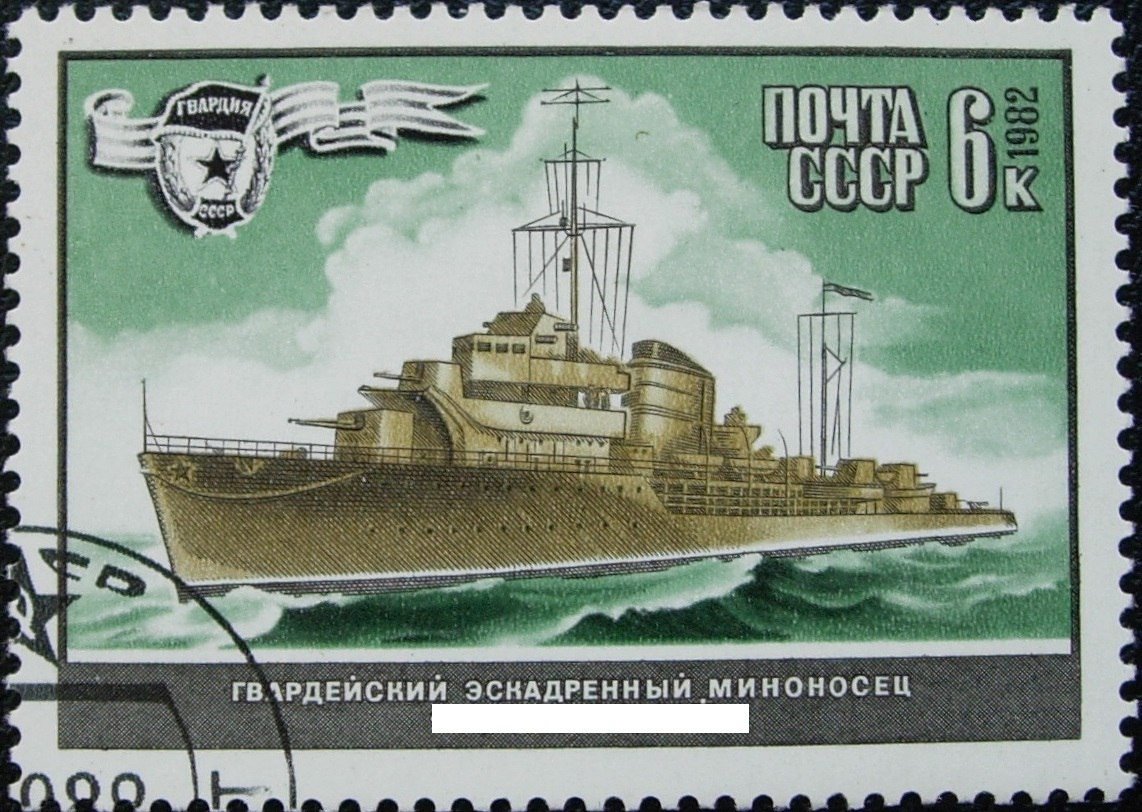
\includegraphics{chapter/ship/Secret_Grem_ship.jpg}}
	  }
	Ответ: \href{https://ru.wikipedia.org/wiki/Гремящий_(эсминец,_1937)}{Гремящий (эсминец, 1937)}.
\end{task}


\begin{task}
	\label{answer:ship_2}
	\newthought{Исходя из графика зависимости кораблей и военных действий (Рис. \ref{fig:ships_by_country_and_conflict}), на какую страну приходится больше всего значений войн, с которыми связаны корабли?
	\begin{itemize}
	  \item СССР
	  \item Россия
	  \item Российская Империя
	\end{itemize}}
	Ответ: СССР.
\end{task}


\begin{task}
	\label{answer:ship_3}
	\newthought{Исходя из этого же графика, на какую войну приходится больше всего значений кораблей?
	\begin{itemize}
	  \item \href{https://www.wikidata.org/wiki/Q159950}{Русско-японская война}
	  \item \href{https://www.wikidata.org/wiki/Q362}{Вторая мировая война}
	  \item \href{https://www.wikidata.org/wiki/Q254106}{Крымская война}
	\end{itemize}}
	Ответ: вторая мировая война.
\end{task}

